\documentclass[10pt,a4paper]{extarticle}
\usepackage[latin1]{inputenc}
\usepackage{amsmath}
\usepackage{microtype}
\usepackage[none]{hyphenat}
\usepackage{verbatim}
\usepackage{amsfonts}
\usepackage{amssymb}
\usepackage{enumitem}
\renewcommand{\familydefault}{\sfdefault}
\usepackage{mathpazo}
\renewcommand{\rmdefault}{put}
\usepackage{enumitem}
\usepackage[dvipsnames,svgnames]{xcolor}
\usepackage{tkz-euclide}
\usetkzobj{all}
\usepackage{graphicx}
\usepackage{tikz} 	
\usepackage{adjustbox}
\usepackage{multicol}
\usepackage{lipsum}
\usepackage[left=0.7cm,right=1cm,top=1cm,bottom=1.5cm]{geometry}
\usepackage{cancel} \usepackage{xcolor}
\usepackage{tcolorbox}
\usetikzlibrary{decorations.pathmorphing,patterns}
\usetikzlibrary{decorations.pathreplacing,calc}
 \newcommand\coret[2][red]{\renewcommand\CancelColor{\color{#1}}\cancel{#2}}
\SetLabelAlign{Center}{\hfil\makebox[1.0em]{#1}\hfil}

%%_------= solusi


% Set this =0 to hide, =1 to show

% Set this =0 to hide, =1 to show
\newtcolorbox{mybox}[1][] { colframe = blue!10, colback = blue!3,boxsep=0pt,left=0.2em, coltitle = blue!20!black, title = \textbf{jawab}, #1, } 

%---------- kunci (jika 1 ) muncul
\def\tampilkunci{1}
\newcommand{\hide}[1]{\ifnum\tampilkunci=1
%
\begin{mybox}
 #1
\end{mybox}
%
\vspace{\baselineskip}\fi}



\newcommand*\cicled[1]{\tikz[baseline=(char.base)]{\node[white, shape=circle, fill=red!80,draw,inner sep=0.5pt](char){#1};}}

\newcommand*\kunci[1]{\ifnum\tampilkunci=1
%
\tikz[baseline=(char.base)]{\node[red, shape=circle,draw,inner sep=0.5pt,xshift=2pt](char){#1};}\stepcounter{enumii}
\fi\ifnum\tampilkunci=0
%
\hspace{3pt}#1\stepcounter{enumii}
%
\fi}

\newcommand*\silang[1]{\tikz[baseline=(char.base)]{
\draw[red,thick](-0.2,-0.20)--(0.2,0.2);
\draw[red,thick](-0.2,0.20)--(0.2,-0.2);
\node[black](char){#1};
}}

\newcommand*\centang[1]{\tikz[baseline=(char.base)]{
\draw[red, very thick](-0.2,0.1)--(-0.1,0)--(0.2,0.3);
\node(char){#1};
}}

\newcommand*\merah[1]{
\textcolor{red}{#1}}
\newcommand*\pilgan[1]{
\begin{enumerate}[label=\Alph*., itemsep=0pt,topsep=0pt,leftmargin=*,align=Center] #1 
\end{enumerate}}
\newcommand*\pernyataan[1]{
\begin{enumerate}[label=(\arabic*), itemsep=0pt,topsep=0pt,leftmargin=*] #1 
\end{enumerate}}

\newcommand*\daftar[1]{
\begin{itemize}[label=$\bullet$, itemsep=0pt,topsep=0pt,leftmargin=*] #1 
\end{itemize}}


\newcommand{\pilgani}[1]{                            \vspace{-0.3cm}\begin{multicols}{2}
 \begin{enumerate}[label=\Alph*., itemsep=0pt,topsep=0pt,leftmargin=*,align=Center]#1                     \end{enumerate}
 \phantom{ini cuma sapi, wedus, dan ayam}
 \end{multicols}}


\begin{document}


 \textbf{Ringkasan dan Latihan Momentum} \phantom{ini nama siswa yang aaamengerjakan soal kuis ini }  

\begin{multicols*}{2}
\textbf{Momentum}

Momentum adalah tingkat kesulitan kesulitan untuk menghentikan benda. Faktor yang mempengaruhi adalah $m$ (massa) dan $v$ (kecepatan)

$$ p = m v \text{  (Ns)}$$

Momentum bersifat vektor, sehingga memperhatikan arah ( + / - ) dan sudut vektor 


\begin{enumerate}
\item Sebuah benda kecepatannya 20 m/s, dengan massa 1000 kg. Maka momentum benda tersebut adalah 
\pilgani{
        \item 10.000 Ns
        \item 20.000 Ns
        \item 30.000 Ns
        \item 40.000 Ns
        \item 50.000 Ns
        }
\item Bola A bermassa 2 kg bergerak ke sumbu-$x$ dengan kecepatan 20 m/s dan bola B dengan massa 1 kg bergerak ke sumbu-$y$ 30 m/s. Jumlah momentum kedua benda adalah . . .
\pilgani{
        \item 70 Ns
        \item 10 Ns
        \item -10 Ns
        \item 50 Ns
        \item 20 Ns
        }

\item Balok A bermassa 1 kg bergerak ke sumbu-$x$ dengan kecepatan 10 m/s, balok B bermassa 3 kg bergerak dengan kecepatan sama ke arah 30$^o$ dari sumbu-$y$. Total momentum kedua benda tersebut adalah . . .
\pilgani{
        \item $10\sqrt{10+1,5\sqrt{3}}$
        \item $10\sqrt{13}$
        \item $10$
        \item $40$
        \item -20
        }
\vspace{3cm}
\textbf{Kekekalan Momentum}

\begin{align*}
\Sigma p &= \Sigma p'\\
m_1.v_1 + m_2.v_2 &= m_1.v_1' +m_2v_2'\\
\end{align*}

\item Dua benda A dan B masing-masing massanya 4 kg dan 5 kg. Mereka bergerak dengan kecepatan berlawanan. Kecepatan A adalah 6 m/s, dan kecepatan B adalah $v$. Jika setelah bertumbukan, benda A dan B berbalik arah dengan kecepatan 4 m/s dan 2 m/s maka kecepatan awal B adalah . . . 
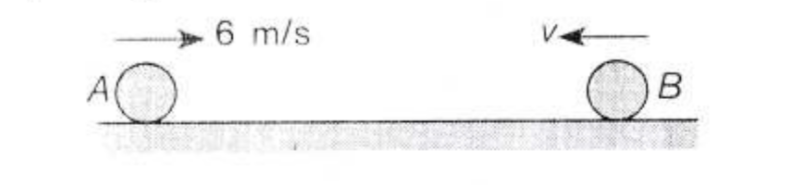
\includegraphics[width=8cm]{pic/mom1}
\pilgani{
        \item 6 m/s
        \item 3 m/s
        \item 1,6 m/s
        \item 1,2 m/s
        \item 0,4 m/s
        }
\vspace{2cm}

\item Benda bermassa 0,5 kg bergerak ke timur 2 m/s, tabrakan dengan benda lain 0,3 kg m/s ke barat. Setelah tabrakan benda 0,3 kg bergerak 2 m/s ke timur. Berapa kecepatan benda 0,5 kg? . . . . arahnya ke . . . .
\vspace{2cm}


\textbf{Jenis tumbukan, koefisien restitusi $e$}
        \begin{enumerate}
\item Lenting sempurna
     \daftar{
        \item $e =1 $
        \item $\Sigma p = \Sigma p' $
        \item Energi kinetik kekal $EK=EK'$
        }

 \item Lenting Sebagian
        \daftar{
        \item $0<e<1$
        \item $\Sigma p = \Sigma p'$
        \item $EK> EK'$ artinya ada energi kinetik yang hilang, menjadi energi lain (misal: bunyi, panas, perubahan bentuk \textit{defomasi}}

 \item Tidak lenting sama sekali
        \daftar{
        \item $e=0$
        \item $\Sigma p = \Sigma p'$
        \item setelah bertumbukan kedua benda menjadi satu, sehingga 
        \item $m_Av_A + m_Bv_B = (m_A + m_B)v'$
        }
        \end{enumerate}

Koefisien restitusi

$$ e = \frac{-(v_2'-v_1')}{v_2-v_1} = \sqrt{\frac{h'}{h}} $$
$$ v = \sqrt{ 2gh}$$
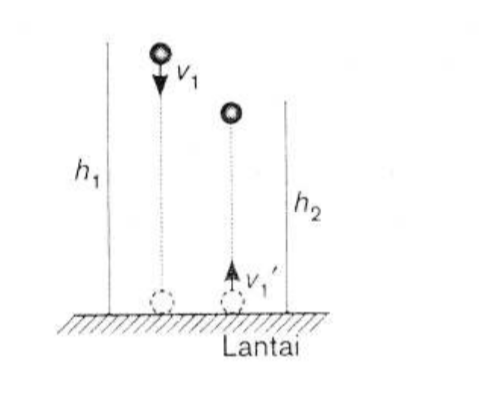
\includegraphics[height=5cm]{pic/mom2}

Keterangan:

$v_1'$, $v_2'$ adalah kecepatan akhir\\
$v_1$, $v_2$ kecepatan awal\\
$h'$ ketinggian akhir, $h$ ketinggian awal\\

\item[ex] Dua buah benda dengan massa sama, 0.1 kg bergerak dengan kecepatan 10 m/s dan 8 m/s saling mendekat. Jika terjadi lenting sempurna tentukan kecepatan masing-masing setelah tumbukan

\vspace{1cm}
\hide{
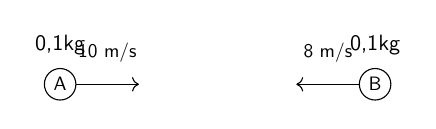
\begin{tikzpicture}
\foreach \x /\y/\z in {0/A/{0,1kg},4/B/{0,1kg}} {
\draw (\x,0) circle (0.2) node[scale=0.7]{\y};
\node at (\x,0.5) [scale=0.8]{\z};}
\draw[->] (0.2,0)--node[midway, yshift=0.4cm,scale=0.7]{10 m/s}(1,0);
\draw[->] (3.8,0)--node[midway, yshift=0.4cm,scale=0.7]{8 m/s}(3,0);
\end{tikzpicture}

Diketahui:

\begin{tabular}{p{0.5cm} p{1mm} p{2cm} p{1cm} p{0.5cm} p{2cm} }
$m_A$ &= &0.1 kg  & & &\\
$m_B$ &= &0.1 kg  & & &\\
$v_A$ &= &10 m/s  & & &\\
$v_B$ &= &-8 m/s  & & &\\
$e$ &= &1  & & &\\
\end{tabular}

Ditanya : $v_A'$ atau $v_1'$ dan $EK_A'$ ?

Jawab:

Karena lenting sempurna maka berlaku
\begin{align*}
e &= \frac{-(v_2'-v_1')}{v_2-v_1}\\
1 &= \frac{-v_2'+v_1'}{-8-(10)}\\
1 &= \frac{-(v_2'-v_1')}{-18}\\
\coret{-}18 &= \coret{-}(v_2'-v_1')\\
18 &= v_2' -v_1'
\end{align*}
Berlaku pula persamaan kekekalan momentum, massa sama
\begin{align*}
\Sigma p &= \Sigma p\\
\coret{m_A}v_1 + \coret{m_B}v_2 &= \coret{m_A}v_1' + \coret{m_B}v_2' \\
10-8 &= v_1' + v_2'\\
2 &= v_1' + v_2'
\end{align*}
Kemudian proses eliminasi sehingga 
\begin{align*}
18 &= v_2' -v_1'\\
2 &= v_2' + v_1'\\
\text{----}&\text{----------------(-)}\\
16 &=-2v_1'\\
v_1' &= -8 \text{ m/s}
\end{align*}
energi Kinetiknya $\frac{1}{2}mv^2=3,2$ J

Jika mereka \textbf{MASSA SAMA dan LENTING SEMPURNA} maka hanya bertukar kecepatan. Sehingga $v_1'=v_2=-8$ dengan arah ke kiri. }

\item Sebuah benda berada pada ketinggian 80 cm. Setelah tumbukan benda memantul. Jika koefisien restitusi benda dan lantai adalah 0,2, maka ketinggian setelah pantulan adalah . . .
\vspace{2cm}


\item Berdasarkan soal sebelumnya, dengan koefisien 0,2 maka kecepatan sesaat setelah pantulan adalah . . . 
\vspace{2cm}



\item Benda A dengan massa 2 kg bergerak ke arah kanan dengan kecepatan 3 m/s bergerak menabrak benda B bermassa 1 kg yang sedang diam. Jika tumbukan yang terjadi adalah tumbukan lenting sempurna, maka kecepatan masing-masing adalah . . . 
\pilgani{
        \item 1 m/s dan -4 m/s
        \item 4 m/s dan 1 m/s
        \item 1 m/s dan 4 m/s
        \item 1,5 m/s dan 2 m/s
        \item -1 m/s dan 2 m/s
        }

\vspace{4cm}

\item Benda A dan B berturut-turut massanya 2 kg dan 1 kg dengan kecepatan saling mendekat dengan kecepatan $v_A$ = 4m/s dan $v_B$ = 1 m/s. Jika kemudian kedua benda bertumbukan lenting sebagian dengan koefisien restitusi diketahui 0,5, maka kecepatan benda B setelah bertumbukan adalah . . .
\pilgani{
        \item 8 m/s
        \item -8 m/s
        \item 6 m/s
        \item -6 m/s
        \item 4 m/s
        }
\vspace{4cm}




\textbf{ Impuls }\\
Impuls adalah gaya selama waktu tertentu menyebabkan perubahan momentum. Jika ditulis sebagai persamaan
$$ I = F.\Delta t = \Delta p = m(v'-v)$$
Impuls juga dapat diperoleh dengan menghitung luas grafik $F-\Delta t$. Luas di atas sumbu $x$ dikurangi luas di bawah sumbu $y$.
\begin{center}
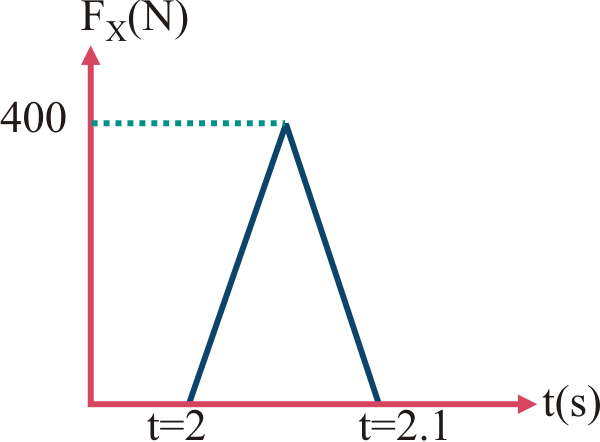
\includegraphics[height=3cm]{pic/impuls}
\end{center}
\item Di atas suatu bidang licin diletakkan balok bermassa 1 kg dalam keadaan diam. Kemudian balok tersebut dikenai gaya tetap 2 N selama 2 sekon. Jika faktor gaya gesekan diabaikan, maka kelajuan balok sesaat setelah gaya dihilangkan adalah . . . .(dalam m/s)
\pilgani{
        \item 4,0
        \item 3,5
        \item 3,0
        \item 2,5
        \item 2,0}

\vspace{2cm}


\item Sebuah mobil bak bermassa 2.000 kg melaju dengan kecepatan 10 m/s menabrak tembok jembatan dalam waktu 0,1 detik. Gaya rata-rata pada mobil selama berlangsungnya tabrakan adalah . . .
\pilgani{
        \item 2$\times 10^2$ N
        \item 2$\times 10^3$ N
        \item 2$\times 10^4$ N
        \item 2$\times 10^5$ N
        \item 2$\times 10^6$ N
        }

\vspace{2cm}



\item Bola bekel massanya 200 gram dijatuhkan dari ketinggian 80 cm tanpa kecepatan awal. Setelah menumbuk lantai, bola bekel memantul kembali dengan kecepatan 1 m/s. Impuls yang terjadi pada saat bola mengenai lantai adalah . . . 
\pilgani{
        \item 1,6 Ns
        \item 1,5 Ns
        \item 1,0 Ns
        \item 0,8 Ns
        \item 0,6 Ns
        }
\vspace{2cm}


\item Impuls yang dibutuhkan untuk menambah kecepatan sebuah mobil yang bermassa 100 kg dari 36 km/jam menjadi 108 km/jam adalah . . .
\pilgani{
        \item 1.000 Ns
        \item 2.000 Ns
        \item 3.000 Ns
        \item 4.000 Ns
        \item 5.000 Ns
        }
\vspace{2cm}


\item Seorang nelayan naik perahu yang bergerak dengan kecepatan 4 m/s. Massa perahu dan orang masing-masing 200 kg dan 50 kg. Pada suatu saat orang tadi meloncat dari perahu dengan kecepatan 8 m/s searah gerak perahu. Kcepatan perahu sesaat orang tadi meloncat adalah . . .
\pilgani{
        \item 1 m/s
        \item 2 m/s
        \item 3 m/s
        \item 4 m/s
        \item 6 m/s
        }
\vspace{5cm}

\item Balok dengan massa 49,9 kg digantung dengan tali sepanjang 1,5 m. Pada saat itu peluru dengan massa 0,1 kg ditembakkan dan bersarang dalam balok sehingga naik 5 cm. Kecepatan peluru sebelum menumbuk adalah . . .

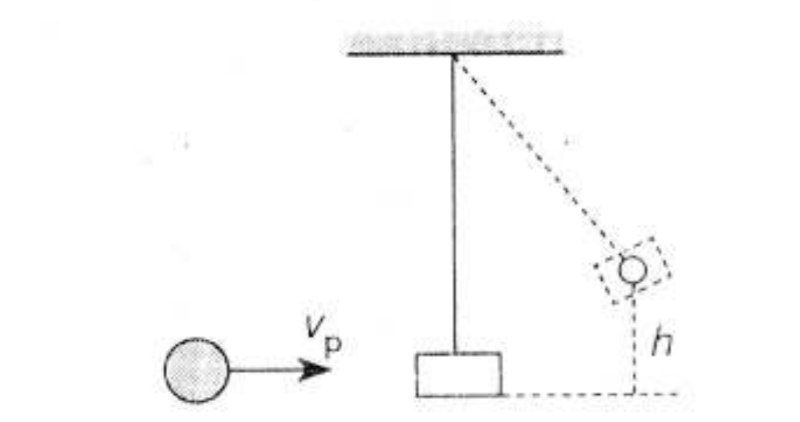
\includegraphics[width=8cm]{pic/mom3}

\pilgani{
        \item 0,5 m/s
        \item 5 m/s
        \item 50 m/s
        \item 500 m/s
        \item 5000 m/s
        }


\end{enumerate}



\end{multicols*}\end{document}


